% Shared standalone design for the editable figure reconstructions.
\documentclass[tikz,border=5pt,10pt]{standalone}
\usepackage[T1]{fontenc}
\usepackage[utf8]{inputenc}
\usepackage{newpxtext,newpxmath}
\usepackage[scaled=.94]{sourcesanspro}
\usepackage{pgfplots}
\pgfplotsset{compat=1.18}
\usetikzlibrary{arrows.meta,calc,positioning,decorations.pathreplacing,
  decorations.markings,patterns,matrix,shapes.geometric,fit,backgrounds,
  intersections,angles,quotes}
\definecolor{ink}{HTML}{203746}
\definecolor{accent}{HTML}{146C78}
\definecolor{muted}{HTML}{667780}
\definecolor{signalred}{HTML}{B94B44}
\color{ink}
\tikzset{>=Latex,line width=.8pt,
  every node/.style={font=\small},
  axis/.style={->,draw=muted,line width=.5pt},
  guide/.style={draw=muted,dashed,line width=.45pt},
  curve/.style={draw=accent,line width=1pt},
  marker/.style={circle,fill=accent,inner sep=1.5pt},
  labelbox/.style={fill=white,inner sep=2pt}}

\begin{document}
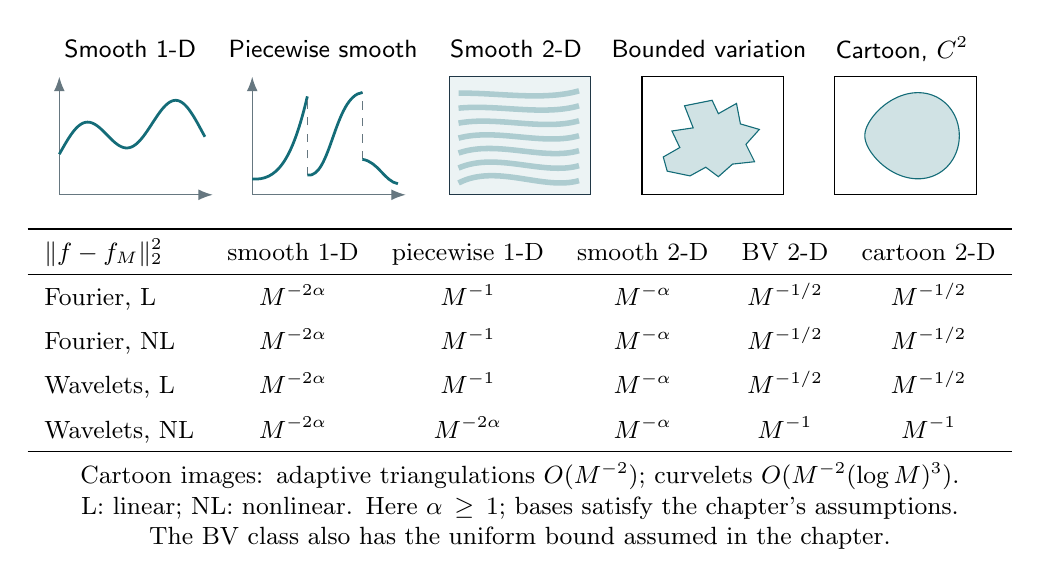
\begin{tikzpicture}[x=1cm,y=1cm]
\foreach \a/\title in {0/{Smooth 1-D},2.45/{Piecewise smooth},4.9/{Smooth 2-D},7.35/{Bounded variation},9.8/{Cartoon, $C^2$}}{
 \node[align=center,font=\small\sffamily] at (\a+1,2.35) {\title};
}
\begin{scope}[shift={(.1,.5)}]
\draw[axis] (0,0)--(1.95,0);\draw[axis](0,0)--(0,1.5);
\draw[curve,domain=0:1.85,samples=100] plot (\x,{.7+.28*sin(300*\x)+.24*sin(110*\x-50)});
\end{scope}
\begin{scope}[shift={(2.55,.5)}]
\draw[axis](0,0)--(1.95,0);\draw[axis](0,0)--(0,1.5);
\draw[curve](0,.2)..controls(.3,.18)and(.5,.4)..(.7,1.25);
\draw[guide](.7,.25)--(.7,1.25);
\draw[curve](.7,.25)..controls(1,.2)and(1.04,1.25)..(1.4,1.3);
\draw[guide](1.4,.45)--(1.4,1.3);
\draw[curve](1.4,.45)..controls(1.6,.42)and(1.68,.17)..(1.85,.14);
\end{scope}
\begin{scope}[shift={(5.05,.5)}]
\path[fill=accent!8,draw=ink] (0,0)rectangle(1.8,1.5);
\foreach \j in {0,...,6}{\draw[accent!35,line width=2pt] (.12,{.15+.19*\j})..controls(.6,{.4+.15*\j})and(1.2,{.05+.19*\j})..(1.65,{.18+.19*\j});}
\end{scope}
\begin{scope}[shift={(7.5,.5)}]
\draw (0,0) rectangle(1.8,1.5);
\path[fill=accent!20,draw=accent] (.32,.3)--(.27,.48)--(.48,.6)--(.38,.81)--(.65,.85)--(.54,1.13)--(.89,1.2)--(.97,1.03)--(1.2,1.16)--(1.25,.9)--(1.49,.83)--(1.32,.64)--(1.43,.42)--(1.15,.39)--(.97,.23)--(.81,.35)--(.61,.24)--cycle;
\end{scope}
\begin{scope}[shift={(9.95,.5)}]
\draw (0,0) rectangle(1.8,1.5);
\path[fill=accent!20,draw=accent] plot[domain=0:360,samples=121] ({.9+.6*cos(\x)+.08*cos(2*\x)},{.75+.5*sin(\x)+.12*sin(2*\x)})--cycle;
\end{scope}
\node[anchor=north,inner sep=0] at (5.95,.08) {\renewcommand{\arraystretch}{1.45}\begin{tabular}{lccccc}
\hline
$\|f-f_M\|_2^2\lesssim$ & smooth 1-D & piecewise 1-D & smooth 2-D & BV 2-D & cartoon 2-D\\\hline
Fourier, L & $M^{-2\alpha}$ & $M^{-1}$ & $M^{-\alpha}$ & $M^{-1/2}$ & $M^{-1/2}$\\
Fourier, NL & $M^{-2\alpha}$ & $M^{-1}$ & $M^{-\alpha}$ & $M^{-1/2}$ & $M^{-1/2}$\\
Wavelets, L & $M^{-2\alpha}$ & $M^{-1}$ & $M^{-\alpha}$ & $M^{-1/2}$ & $M^{-1/2}$\\
Wavelets, NL & $M^{-2\alpha}$ & $M^{-2\alpha}$ & $M^{-\alpha}$ & $M^{-1}$ & $M^{-1}$\\\hline
\end{tabular}};
\node[align=center,text width=12cm] at (5.95,-3.45) {Cartoon images: adaptive triangulations $O(M^{-2})$; curvelets $O(M^{-2}(\log M)^3)$.\\L: linear; NL: nonlinear. Here $\alpha\geq1$; bases satisfy the chapter's assumptions.\\The BV class also has the uniform bound assumed in the chapter.};
\end{tikzpicture}
\end{document}
